\documentclass[11pt]{article}
\usepackage{hyperref}
\usepackage{graphicx}
\usepackage{amsmath}
\usepackage{amsfonts}
\usepackage{fullpage}
\usepackage{fontspec}
\usepackage{hyperref}
\setmainfont[Ligatures=TeX]{Arial.ttf}

%\usepackage{helvet}
%\renewcommand{\familydefault}{\sfdefault}
\title{The Higgs Boson Decay Classification}    
%\date{}
\author{
  He, Qiyang\\
  \and
  Wang, Xiaoying\\
  \and
  Weng, Jeff\\
}  
\begin{document}
\maketitle
% By creating a machine learning model


\renewcommand{\abstractname}{\large{\textbf{Abstract}}}
\begin{abstract}
The Higgs Boson has many different processes through which it can decay. The classification of these processes may help physicists to explore the nature of the Higgs Boson’s interaction with other particles. In order to accurately determine whether a Higgs Boson is decaying into tau particles (a type of lepton) within a particle accelerator or decaying into other particles, we employ several linear and non-linear models as well as machine learning methods to achieve an ideal classification. We use ROC score, AMS together with Cross Validation accuracy to compare the models, among which Random Forest with 1000 trees and 20 max-depths performs the best with the highest accuracy rate of 0.838.\\
%\textbf{Keywords:} aaa, bbb

\end{abstract}



\section*{1\quad Introduction}
Our study is based on the Higgs Boson Machine Learning Challenge carried out by Kaggle and CERN. The challenge was organized to promote collaboration between high energy physicists and data scientists by releasing a portion of the simulated data used by physicists to optimize the analysis of the Higgs Boson. The participants were encouraged to find a region in the feature space that could highly separate the signals and the background.    

\subsection*{1.1\quad Physical background}
The Higgs Boson particle is a fundamental particle in our understanding of our universe as physicists believe that it is the particle that generates mass when interacting with other particles. Because of this, physicists are running experiments to confirm its existence and to accurately classify it. Our data is collected from simulations of colliding two protons at high energy. When this happens, the protons break apart into gluons and quarks and form conic structures called jets. The jets, as well as other characteristics of the collision, are then measured to study the properties of the resulting particles.

Because quarks and gluons are unstable particles when by themselves, they will interact with other particles to form or decay into new types of particles. One specific particle, the Higgs Boson particle decays into two tau particles, which the experiment tries to measure. Using different measurements obtained during the simulations as features, we attempt to predict whether or not an event is the tau tau decay of a Higgs Boson particle or simply background noise.

\subsection*{1.2\quad Previous studies}
There are three ways to classify a particle discovery in high energy physics (HEP). In a partial physical experiment, assume we are measuring p quantities for each events, which can be written as x=($x_{1}$,...,$x_{p}$). In our specific case $x_{1}$ could represent the missing transverse energy, $x_{2}$ could represent the invariant mass of the hadronic tau and the lepton, and so on. We can set probability density functions for both signal and background events as $f(x|s)$, $f(x|b)$. In order to select or define a selection region for signal events, making cuts on variables are a common practice in HEP. The simple process may require physical intuition in determining the value of the cuts (Adam-Bourdarios et al., 2014).   

Other ways to execute classifications are using a linear boundary or non-linear boundary. Specially, in order to exploit the potential sophisticated shapes of the pdfs $f(x|s)$,$f(x|b)$, a non-linear boundary is necessary. If using contours of constant likelihood ratio, an optimal boundary for event classification is obtained as below, according to Neyman-Pearson lemma(Kendall et al., 1987). $$\lambda(x)=\frac{f(x|s)}{f(x|b)}$$

Because both of the $f(x|s)$, $f(x|b)$ are unknown in close form, generally we can't speculate $\lambda(x)$ at point x. However, if we use specific Monte-Carlo models to generate samples for signals and background processes, we can use Machine Learning methods to define $y(x)$ which can best approximates the likelihood ratio or a monotonic function. In the Higgs Boson Challenge, unlike many HEP problems, both signals and background processes are already known to exist, so the problem is boils down to a classification problem.

Multivariate methods like Fisher discriminants and neural networks used to play a pivotal roles in HEP to solve such problems described above. However, recently advanced machine learning methods like Support Vector Machine (SVM) and Adaboosting are slowly spreading into HEP research fields. A special objective function AMS\footnote{Approximate Median Significance, detailed information is introduced in "Method" Section} is often used for evaluating the classifying results in HEP research.


In Higgs Boson Machine Learning Challenge, ensemble methods and individual methods are used in order to achieve a high score for classification. The winning team(G. Melis, 2015) used DNN which was an ensemble of 70 neural networks whose predicted probabilities were combined by simple arithmetic averaging. Their AMS score was 3.81. Regularized Greedy Forest was applied by second winner, who used a variation on gradient boosting that decouples structure search and optimization. Their final solution combines multiple RGF through stacking, with a linear regression as the learning model. Other popular methods like Naive Bayes, XGBoost, SVM and Deep Learning were widely in use during the competition. Methods like K-nearest-neighborhood, SVM are proved to be hard to perform significantly better than Boosting (S. Raza Ahmad, 2014), which had an approximate accuracy rate of around 0.83 and an average AMS score of 2.1 on the data set with around 500k events. 

\subsection*{1.3\quad Expectations}
%The trend of the challenge is mainly ensemble methods, deep neural networks and advanced tree-based algorithms. However, there exists opinions that(higgs boson ml challenge t28) the usage of novel algorithms and handling different features may have less effect compared with having a slow but steady learning rate and running the same algorithms iteratively. % Finally, a arguably and futuristic question is whether deep learning could be used to improve the discovery significance. Pertinent research( baldi 2014) gave positive hint when looking for exotic particles.

Based on the methods used in Higgs Boson Challenge together with the arguments above, we decide to use several linear and non-linear machine learning methods to set boundary for our selection region, in order to maximize our prediction accuracy and obtain relatively justifiable AMS score. Special attention will be paid onto Random Forest with advanced hyper-parameters and several boosting methods. Contrasts will be made between linear approaching, Boosting, SVM as well as other machine learning algorithms by their performances of prediction rate and AMS score.

\vspace{30pt}

\section*{2 \quad Methods\footnote{We use R to accomplish EDA and PCA, and Python to do most of the classifications. Because of the large computation complexity we used the Gandalf server in University of California, Berkeley to accomplish the Random Forest fitting. Specific code files please refer to Supplementary Methods offered with the paper.}}

This section mainly explains our data, the objective function AMS and the nature of linear \& non-linear models we decided to apply onto our data.

\subsection*{2.1\quad The Data }
Our data is a sample of the entire Higgs Boson Challenge data set\footnote{The link of the whole dataset: \url{http://opendata.cern.ch/record/328} }. Due to the computational complexity and the limitation of time, we took a sub model which included 50000 observations. The final dataset included 30 features, a weight column used for computing AMS and a label column which denoted whether the event was "signal"( the decay of H $\rightarrow$ $\tau^{+}\tau^{-}$ ) or "background"(other types of decay that is not of interest in this case).

Before doing some real analysis, some EDA procedures were applied. We decide to try to detect missing values in the data set. Variables were denoted as “may be undefined” when they are meaningless or cannot be computed. For example, if an attribute is related to a particular jet, and if no jets are present, then the value cannot not exist and is thus denoted as "may be undefined".  In our data set, their value is -999.0, which is outside the normal range of all variables. These values are regarded as missing value.

In order to execute our classification process sensibly, we used PCA to give a low-dimensional visualization and to achieve dimension reduction before using some machine learning methods. 

\subsection*{2.2\quad The AMS}
The AMS is an objective function used to decide a region in the feature space where one expects an enhanced number of signal events. This function is widely used in optimizing the selection region for discovery significance in HEP research. In the Higgs Boson Challenge, it is being used to score different models. The AMS is defined as follows\footnote{
For specific derivation of AMS please refer to Appendix.1}  
$$AMS_{0}=\sqrt{2\bigg(\big(s+b\big)log\big(1+\frac{s}{b}\big)-s\bigg)}$$ 

In our case we use $$AMS_{1}=\frac{s}{\sqrt{b}}$$ for substitution of our test metric, because when $b\gg s$ (which is the situation in this case) these two are roughly identical. Apart from comparing models' prediction appearance, we will also be comparing their AMS scores to evaluate their performances. In practice, the data samples are finite and the estimates of s and b are themselves subject to some statistical uncertainty. We will do the AMS computation for a certain kind of model after we obtain the best-performing classifier of that kind.


\subsection*{2.3\quad The Models}
\subsubsection*{2.3.1\quad Linear Model}
Several linear models are employed in this case. Because the response variable is binary, for each $\mu$ in
$$\mu_{i}=\beta_{0}+\beta_{1}x_{i1}+...+\beta{p}x_{ip}$$ 
 a unit increment in x does not linearly cause $\beta_{j}$ unit increase in $\mu_{i}$ when other $\beta$ are unchanged. Instead, the increment is a function related to $\mu$ which is called link function. We use logistic regression in this case, rather than Gaussian-based OLS or GLS. 

In order to improve prediction error by shrinking large regression coefficients to reduce overfitting, we introduced LASSO and Ridge to logistic models. By adding constrains like $\lambda||\beta||^{2}_{2}$ onto the term$||Y-x\beta||^{2}$, we derive a Ridge-based biased estimator$\beta=(X^{T}X+\lambda I)^{-1}X^{T}Y$ which is under certain penalty.

LASSO can both overcome overfitting and also perform covariate selection and therefore help make the model more interpretable. It forces certain coefficients to be set to zero, effectively choosing a simpler model that does not include those coefficients. The object of LASSO is to solve $argmin||Y-X\beta||^{2}$ subject to $\sum^{p}_{i=0}||\beta_{i}||\leq C$. We plan to use cross validation to find the ideal $\lambda$.

\subsubsection*{2.3.2\quad Non-Linear Model}
We also use several non-linear models in order to classify the data. Apart from calculating the prediction rate, the ROC score and AMS score will also be computed for comparison.

The first choice is Random Forest model with advanced hyper-parameters. Random Forest is an ensemble machine learning model which is combines the quantities of multiple decision trees. In our case we use the "gini" criterion and set the tree number as a variable in order to optimize the prediction performance.

K-nearest-neighborhood is also frequently used for classification problems. We use Euclidean distance to make the computations. An object is classified by a majority vote of its neighbors. The distance between event j and k is $$d(j,k)=\sqrt{\sum^{p}_{i=1}(x_{ij}-x_{ik})^{2}}$$ Due to the sensitivity of KNN in high dimensional data, we used PCA to apply a feature extraction process before classification. 

Boosting is a newly developed algorithm for classification. In this case we use Adaptive Boosting and Gradient Boosting, which identifies ‘shortcomings’ (of existing weak learners) by high-weight data points and by gradients, respectively.

We will also apply Support Vector Machine on our dataset. We chose both linear and radial kernelized SVM to make comparisons. SVM is workable especially for high-dimensional data. In our case we don't need feature reduction before processing this method.

We also use Deep Learning and Naive Bayes to compare the classification performance. Specific hyper-parameters are shown in the result section.

%i). K-nearest-Neighborhood

%This method is widely used in the Higgs Boson challenge. The basic mechanism of this classification method is to compute the distance between an event and the nearby cases to get several nearby "neighbors". Here we use Euclidean distance to make computations. By taking different odd number of "neighbors", an object is classified by a majority vote of its neighbors. The distance between event j and k is $$d(j,k)=\sqrt{\sum^{p}_{i=1}(x_{ij}-x_{ik})^{2}}$$
%Considering a high dimension in our data set as well as the "curse" of dimensionality for knn (all vectors are almost equidistant to the search query vector when computing Euc-distance in high dimensions), we decide to execute a feature extraction process, which is PCA to achieve the dimension reduction.\\

%ii). Boosting 

%Boosting is a newly developed and highly-used method for classification and machine learning. In this case we use two different boost which is Adaptive Boosting and Gradient Boosting. Generally, the difference between these two is the way dealing with the "shortcomings". In Gradient Boosting, ‘shortcomings’ (of existing weak learners) are identified by gradients. In Adaboost, ‘shortcomings’ are identified by high-weight data points. Adaboost could be regarded as a special case of Gradient Boosting in terms of loss function.  

%For Gradient Boosting, the goal is to find a model $\hat{y}=F$ that minimize the mean square error. The gradient boosting has the assumption that in some layer of the classification the model $F_{t}$ may be imperfect, and it improves it by adding a new model $h(x)$ onto the model to provide a better one.

%For AdaBoosting, it chooses the best weak learner in each layer, and given it certain weight. On each layer a new weak learner combined with its weight would be add on to the existing model. 

%The similarity between these two boosting method is they all use the classifier built in the following term $$F_{T}(x) = \sum_{t=1}^T f_{t}(x)$$ where $f_{t}(x) = \alpha_{t}h(x)$ is an individually weak learner. $\alpha_{t}$ is the coefficient and $h_{t}$ is a hypothesis function, in this case $h_{t}:X \rightarrow \{s,b\}$. The boosting continues for T time's iteration in order to get a minimum sum of training error.\\ 

%iii). SVM

%Support Vector Machine is another machine learning methods that analyze data used for classification and regression analysis. SVM can both work for linear and non-linear classification. In this case we decide to try both to compare for the performance.

%In a linear SVM, we would like to find the function with the least (Training Error + Complexity term), which is $$\frac{1}{m}\sum^{m}_{i=1}l(f(x_{i},\alpha),y_{i})+C(x,w)$$ Here $l$ is the zero-one loss function, which means $l(y,\hat{y})=1$, if $y\neq \hat{y}$, and 0 otherwise; $f(x,\alpha)$ is the classifier function and $\alpha$ is the parameter.
%The comp[exity term is related to parameter somehow. We can use $||w_{i}||^{2}$ in this case, which represent a weight vector for each variable in the data set. Under the constrain $y_{i}(w \times x_{i}+b)\geq 1$(b is the noise), we can minimize the total function.

\vspace{30pt}

\section*{3 Results}
\subsection*{3.1 Exploratory Data Analysis}
During this stage, we looked at the distribution of the features based on whether or not they were signal or background noise. We did this by making density plots to see which features were the most dissimilar based on their labels. The distribution of most of the features were very similar for both background and signal events. However the features, PRI\_jet\_num, which quanitifies the number of jets produced during the collision, PRI\_lep\_eta, the psuedorapidity of the lepton, and DER\_mass\_transverse\_met\_lep, the transverse mass between the missing transverse energy
and the lepton had distributions which appear to be quite different\footnote{Please refer to Figure.3 in Supplementary Results section}. 

In addition, we noticed that seven variables have missing values around 70\% of the time and three variables have missing values around 40\% of the time\footnote{Please refer to Table.2 in Supplementary Results section}. After looking into this, we discovered that the variables that had a significant number of missing values were directly related to the number of jets produced during the collision. Most of the missing values of the variables correspond to events with 0 or 1 jets. 

However, it was found that the missing values were not especially significant. We tried using mean, median, random forest predictions and so on to replace the missing values and the prediction rate did not significantly improve when compared to our baseline. It was also noted that many of the benchmarks changed the missing values to NAs and just ran a training model which handled NA values. We decided not to directly exclude these features in order to retain as much information as possible.

As mentioned before, we carried out PCA for some of the models(e.g. KNN). Since the first 8 PCs explained over 80\% of the data\footnote{Please refer to Table.3 in Supplementary Results section}, we generated a new data set with 8 new features constructed by 8 PCs for our classification.

After we applied PCA onto our data set, we plotted the visualization shown below. Red dots represent signals and black dots represent backgrounds. A spatial ellipse was drawn to define a simultaneous 95\% confidence region for first three components.

%%  center figure locating
\begin{figure}[!ht]
\centering
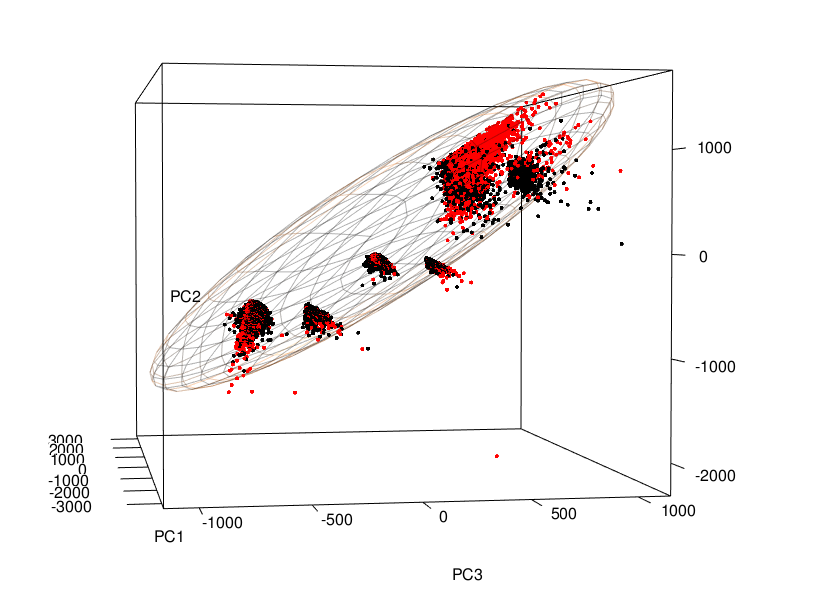
\includegraphics[width=5in]{pca3d.png}
\caption{PCA 3D visualization}
\end{figure}

The signal and background events are merged together in 6 regions within the 3D space. Outliers are explicitly displayed within the area which has relatively high PC2, high PC3 and the area with low PC2 and low PC3. Since most of our features are distributed roughly bell-shaped, we excluded the events exceeding 1.5 times the 95\% range of the given features.

In order to keep consistent scales within our variables to train a predictive model, we normalized our data according to columns before the modelling process.

\subsection*{3.2 Models}

During the prediction stage, we tried 10 different supervised machine learning models on classifying the Higgs Boson particles. The performance of all the models were evaluated by both prediction accuracy and AUC\_ROC scores, using 10-fold cross validation.

Of all the models that we tried, Random Forest with 1000 trees using Gini-index as the splitting criteria worked best with 83.80\% cross validation prediction accuracy and 0.906 AUC\_ROC score, followed very closely by Gradient Boosting Classifier based on `deviance' loss and 100 iterations with 83.4\% prediction accuracy and 0.804 AUC\_ROC score, then by Adaboosting Classifier with 80.6\% prediction accuracy and 0.769 AUC\_ROC score. A bit further behind are K-nearest neighbors with K = 7, which got 79.3\% prediction accuracy and 0.845 AUC\_ROC score, and Deep Learning with 5 hidden layers and 50 neurons in each hidden layer, which got 78.5\% prediciton accuracy and 0.766 AUC\_ROC score. Lasso Logistic Regression, Ridge Logistic Regression, Linear SVM, Radial Kernelized SVM, Naive Bayes did not perform very well in our experiment. None of these five methods got a prediction accuracy over 75\%. In Table 1, we list the cross validation prediction accuracy, AUC\_ROC scores, and values of tuned hyper-parameters of all the 10 models we used on classification. Also see Appendix A.3 Figure 6-13 for the ROC plots of all the models we used.

For all the hyper-parameters in different models, we used 10-fold cross validation to find the best value of each hyper-parameter that would bring the highest average prediction accuracy over 10 times of randomized cross validation. One special case was the boosting algorithms. In either Gradient Boosting Classifier or Adaboosting Classifier, there are two main hyper-parameters: the number of trees (n\_estimators) and the learning\_rate, which control for over-fitting via shrinkage. We tuned these two hyper-parameters with various value combinations. In general, the accuracy increases as the number of estimators increases, and this holds across all learning rates. However, the two hyper-parameters affect each other, and the best combination of parameters appears to be the one with 100 estimators and a learning rate of 0.01 for Gradient Boosting Classifier, and the one with 100 estimators and a learning rate of 0.1 for Adaboosting classifier. Boosting classifiers are then built based on these values.

\begin{table}[!ht]
    \centering
    \begin{tabular}{|c | c c c | }
    \hline
    Model & CV Accuracy & CV AUC\_ROC & Hyper-parameters\\ 
    \hline
    \hline
    LASSO Logistic Regression & 0.747 & 0.811 & penalty = L1, c = 0.1 \\
    \hline
    Ridge Logistic Regression & 0.744 & 0.810 & penalty = L2, c = 1.0 \\
    \hline
    Random Forest & 0.838 & 0.906 &
    \begin{tabular}{@{}c@{}}estimators=1000\\ criterion=`gini'\\ max\_depth=20\\ bootstrap=True\\
    \end{tabular}\\
    \hline
    Linear SVM & 0.550 & N/A & kernel = `linear', c = 0.01\\
    \hline
    Radial Kernelized SVM & 0.663 & N/A & kernel = `rbf', c = 1.0\\
    \hline
    Naive Bayes & 0.624 & 0.652 & alpha = 0.01\\
    \hline
    K-nearest Neighbors & 0.793 & 0.845 & k = 7\\
    \hline
    Gradient Boosting Classifier & 0.834 & 0.804 &
    \begin{tabular}{@{}c@{}}loss=`deviance'\\ n\_estimators=100\\ learning\_rate=0.01\\
    \end{tabular}\\
    \hline
    Adaboosting Classifier & 0.806 & 0.769 & 
    \begin{tabular}{@{}c@{}}n\_estimators=100\\learning\_rate=0.1\\
    \end{tabular}\\
    \hline
    Deep Learning & 0.785 & 0.766 &
    \begin{tabular}{@{}c@{}}activation = `logistic'\\ penalty alpha = 0.00001\\ hidden\_layer\_sizes=50x5layers\\
    \end{tabular}\\
    \hline
    \end{tabular}\\
    \caption{Prediction performance of different Machine Learning models}
    \label{tab:my_label}
\end{table}

As mentioned previously in the methods section, in addition to prediction accuracy and AUC\_ROC score, we also used Approximate Median Significance (AMS) as an extra evaluation metric among out own models. Refer to Section 2.2 - the AMS, for detailed definition and indication of AMS score. Figure 2 shows the AMS scores of all the ten models we used. In accordance with the performance results based on prediction accuracy and AUC\_ROC score, our best model Random Forest got the highest AMS score.

However, the AMS is not always a stable metric. It is largly decided by the data set. According to G. Melis's report\footnote{G. Melis. \textit{Dissecting the winning solution of the higgsml challenge}.2015}, the prediction accuracy and model selection are both severely limited by the amount of data available. It also demonstrated a diminishing performance of AMS score when the data set is shrunk in order to avoid overfitting. A larger data set may be a good trade off for a better AMS performance. Since the size of the dataset we are working on is only 50,000, which is 1/11 of the 550,000 testset used by Kaggle, our AMS score is much smaller than other previously mentioned study groups. But the difference of performance in models will not differ significantly.

\begin{figure}[!ht]
    \centering
    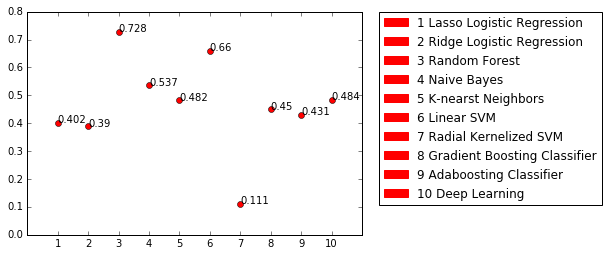
\includegraphics[width=6in]{ams.png}
    \caption{AMS score of different Machine Learning models}
\end{figure}

\vspace{50pt}
\section*{4 Discussion}
Among all the supervised machine learning models, Random Forest performs the best. As the results indicate, ensemble methods are very powerful in classification problems. The full data set originally contained 30 predictors, many of which were likely to be highly correlated. Combining predictions from multiple models in ensembles work better if the predictions from the sub-models are uncorrelated or at best weakly correlated. 
Like to other greedy algorithms that may have highly correlated predictors, like decision trees or even decision trees with bagging, Random Forest is an algorithm that the subtrees are learned so that the resulting predictions from all of the subtrees have less correlation. In addition, theoretically, Random Forest, as a randomized tree-based model, can approximate functions with any "shape", comparing with other models that approximate fixed function shapes, like linear regression, or SVM models. These may be the reasons why Random Forest beat other models in this predicting problem.

Gradient Boosting Classifier was the second best model. It had a prediction accuracy of 83.4\%, which was only 0.4\% lower than that of Random Forest. We expected boosting algorithms to improve our prediction results relatively well, since boosting is an ensemble method that sequentially builds models that try to account for error not accounted for by previous classifiers. However, Gradient Boosting Classifier didn't bring any improvements on Random Forest. Its performance is very close to but still lower than that achieved by using Random Forest without boosting. We hypothesize the reason why boosting didn't improve the prediction accuracy is that boosting algorithm is designed to boost a weak learner that is just better than 1/2 accuracy. As base classifiers get stronger (no longer barely above chance) the scope for boosting to improve things reduces. It is increasingly likely to have over-fitted to errors and outliers, so there is no scope to balance a wide variety of variants.

Under the assumption that there may be some underlying linear relationship between predictors and signal labels, we also tried Logistic Regression with different penalty criterion. Depending on the penalty criteria, logistic regression can perform variable selection, and irrelevant predictors either get eliminated or have very low coefficients that do not influence the outcome. We trained Logistic Regression models with both Norm-1 penalty, namely LASSO logistic regression and Norm-2 penalty, namely Ridge logistic regression. LASSO logistic regression seems to perform slightly better than Ridge logistic regression on this specific problem.

Based on our study, several further studies may be developed in different perspectives of our research. In our case,  bagging appeared to perform better than boosting, and we are interested whether this difference will still hold when the dataset is excessively enlarged. Besides, considering large computational work, we did not try DNN in our case. It is worthwhile to develop more advanced contrast between neutral network and boosting as well as bagging for classification challenge.

\vspace{40pt}

\begin{thebibliography}{19}

\bibitem{atlas} 
C. Adam-Bourdarios, G. Cowan, C. Germain-Renaud, I. Guyon, B. K ́egl, D. Rousseau.
\textit{The Higgs Machine Learning Challenge}.
ATL-SOFT-PROC-2015-044, 2015

\bibitem{decay} 
The ATLAS Collaboration.
\textit{Evidence for higgs boson decays to $\tau+$ $\tau-$ final state with the atlas detector.}
Technical Report ATLAS-CONF-2013-108, November 2013
 
\bibitem{software} 
S. Binet, B. Kegl, and D. Rousseau.
\textit{Software for the atlas higgs machine learning challenge 2014.}
CERN Open Data Portal, 2014


\bibitem{baldi} 
P. Baldi, P. Sadowski, and D. Whiteson.
\textit{Searching for Exotic Particles in High-energy Physics with Deep Learning}. 
Nature Communications, 2014
 
 \bibitem{latexcompanion} 
Kendall M G, Stuart A, Ord J K.
\textit{Kendall’s Advanced Theory of Statistics}. 
New York, NY, USA: Oxford University Press, 1987
 
\bibitem{baldi} 
G. Melis.
\textit{Dissecting the winning solution of the higgsml challenge}. 
JMLR: Workshop and Conference Proceedings, 2015

\bibitem{latexcompanion} 
ATLAS Collaboration.
\textit{Data set from the Higgs Machine Learning Challenge, CERN Open Data Portal}. 
opendata.cern.ch/collection/ATLAS-Higgs-Challenge-2014
 
\bibitem{latexcompanion} 
S. Raza Ahmad.
\textit{ Detailed Technical Report as part of participation in
Higgs Boson Machine Learning Challenge}. 
Department of Mathematics, Lahore University of Management Sciences, 2014
 
\bibitem{latexcompanion} 
Benjamin M. Marlin.
\textit{Missing Data Problems in Machine Learning}. 
Online Available, 2008.  \url{http://www.cs.toronto.edu/~marlin/research/phd_thesis/marlin-phd-thesis.pdf} 


\bibitem{latexcompanion} 
Jocelyn Perez, Ravi Ponmalai, Alex Silver, Dacoda Strack.
\textit{ ML2014: Higgs Boson Machine Learning Challenge}. 
University of California, Irvine, 2014


\end{thebibliography}



\vspace{30pt}

\section*{Author Contributions}
Xiaoying Wang: Created the sub-dataset, trained the prediction machine learning models, calculated prediction accuracy, AUC\_ROC score and AMS score, created the ROC plots, discussed the performances of different models in the Results section, and analyzed the advantage/disadvantage of some important models in the Discussion section.

Qiyang He: Developed literature research, mainly finished Abstract, Introduction, Methods and some part of results and discussion. Executed PCA analysis and accomplish the explanation of AMS.

Jeff Weng: Researched and wrote the physical Background section, created density plots for the exploratory data analysis, investigated missing values, and edited/proofread the report.

\clearpage


%%  center figure locating
%\begin{figure}[h]
%\begin{center}
%\framebox[4.0in]{$\;$}
%\fbox{\rule[-.5cm]{0cm}{4cm} \rule[-.5cm]{4cm}{0cm}}
%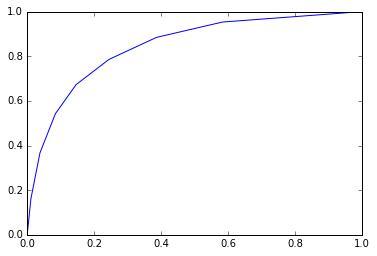
\includegraphics[width=2in]{knn_rocplot.png}
%\end{center}
%\caption{Sample figure caption.}
%\end{figure}

%\vspace{30pt}

\section*{Appendix}

\subsection*{A1. The derivation of AMS}
The AMS is an objective function used to decide a region in the feature space where one expects an enhanced number of signal events. In the real experiment, one could simply counts the number of events "n" found in this region. The number of events found in a region $G$ is assumed to follow a Poisson distribution with mean $\mu_{s} + \mu_{b}$
$$P(n|\mu_{s},\mu_{b})=\frac{(\mu_{s} + \mu_{b})^{n}}{n!}e^{-(\mu_{s} + \mu_{b})}$$
Among which the $\mu_{s}$ and $\mu_{b}$ are the expected numbers of events from the signal and background events. In order to test the existence of eignal event, we set the hypothesis to be $\mu_{s}=0$. We can construct the likelihood ratio as following
$$\lambda=\frac{P(n|0,\mu_{b})}{P(n|\mu_{s},\mu_{b})}=(\frac{\mu_{b}}{n})e^{n-\mu_{b}}$$
In this case, the $\hat{\mu_{s}}=n-\mu_{b}$ is the maximum likelihood estimator of $\mu_{s}$. According to Wilks' theorem(Wilks,1938), we can construct a test statistic under certain condition
$$q0=\[\begin{cases} -2ln\lambda & \text{if } n > \mu_{b}, \\ 0 & \text{otherwise }\end{cases}\]$$

and the p-value of this hypothesis from an observer $q0$ is $$p=1-\Phi(\sqrt{q0})$$
The $\Phi$ is the standard Gaussion cumulative distribution. In particle physics this p value could also be transformed into a metric $Z$ which is $$Z=\Phi^{-1}(1-p)$$ and The Z could also be formed as the following result$$Z=\sqrt{q0}=\sqrt{2\bigg(nln\big(\frac{n}{\mu_{b}}\big)-n+\mu_{b})}$$ 
In our case, we define a search region $G=\{x:g(x)=s\}$ where g is a certain classifer function. So the s and b is the expected number of signal and background events which is defined as below\footnote{Here the function $1\{D\}$ means the value of function is 1 if the argument D is true.} $$s=\sum^{n}_{i=1}w_{i}1\{y_{i}=s\}1\{\hat{y_{i}}=s\}$$ and  $$b=\sum^{n}_{i=1}w_{i}1\{y_{i}=b\}1\{\hat{y_{i}}=s\}$$
If we substitute n with $s+b$ we can get the AMS, which is widely used in HEP to optimize the selection region for discovery significance $$AMS_{0}=\sqrt{2\bigg(\big(s+b\big)log\big(1+\frac{s}{b}\big)-s\bigg)}$$ 
Based on $AMS_{0}$, we can compute the $AMS_{1}$ which is $$AMS_{0}=AMS_{1} \times (1+\mathcal{O}(\frac{s}{b}))$$
$$AMS_{1}=\frac{s}{\sqrt{b}}$$
Specially, When $b\gg s$(which is just the situation in this case) the $AMS_{0}$ and $AMS_{1}$ is indistinguishable close, and this approximation will hold.\\


\clearpage
\section*{Supplementary Results}

\vspace{40pt}

\subsection*{Table.2\quad Missing value percentage}
\begin{table}[!h]
    \centering
    \begin{tabular}{ | c | c | c | c | }
    \hline
    Feature & Percent Missing & Feature & Percent Missing \\ 
    \hline
    \hline
    DER\_mass\_MMC & 0.15362 & PRI\_tau\_phi & 0.00000 \\
    \hline
    DER\_mass\_transverse\_met\_lep & 0.00000 & PRI\_lep\_pt & 0.00000\\
    \hline
    DER\_mass\_vis & 0.00000 & PRI\_lep\_eta & 0.00000\\
    \hline
    DER\_pt\_h & 0.00000 & PRI\_lep\_phi &  0.00000\\
    \hline
    DER\_deltaeta\_jet\_jet & 0.71020 & PRI\_met & 0.00000\\
    \hline
    DER\_mass\_jet\_jet & 0.71020 & PRI\_met\_phi & 0.00000\\
    \hline
    DER\_prodeta\_jet\_jet & 0.71020 & PRI\_met\_sumet & 0.00000\\
    \hline
    DER\_deltar\_tau\_lep & 0.00000 & PRI\_jet\_num & 0.00000 \\
    \hline
    DER\_pt\_tot & 0.00000 & PRI\_jet\_leading\_pt & 0.39984 \\
    \hline
    DER\_sum\_pt & 0.00000 & PRI\_jet\_leading\_eta & 0.39984 \\
    \hline
    DER\_pt\_ratio\_lep\_tau & 0.00000 & PRI\_jet\_leading\_phi & 0.39984 \\
    \hline
    DER\_met\_phi\_centrality & 0.00000 & PRI\_jet\_subleading\_pt & 0.71020 \\
    \hline
    DER\_lep\_eta\_centrality & 0.71020 & PRI\_jet\_subleading\_eta & 0.71020 \\
    \hline
    PRI\_tau\_pt & 0.00000 & PRI\_jet\_subleading\_phi & 0.71020\\
    \hline
    PRI\_tau\_eta & 0.00000 & PRI\_jet\_all\_pt & 0.00000\\
    \hline
    \end{tabular}\\
    \caption{Percentage of missing values for each feature}
    \label{tab:my_label}
\end{table}

\vspace{40pt}



\subsection*{Table.3\quad PCA Importance table}
 \begin{table}[!ht]
     \centering
     \begin{tabular}{|p{1.8cm}|c|c|c|c|c|c|c|c| }
     \hline
       & PC1 & PC2 & PC3 & PC4 & PC5 & PC6 & PC7 & PC8\\ 
     \hline
       Standard deviation & 3.4971 & 1.53827 &1.52661 & 1.40947 & 1.29186 & 1.24495 & 1.09772 & 1.05749\\ 
     \hline
       Variance Proportion & 0.4077 & 0.07888 & 0.07768 & 0.06622 & 0.05563 & 0.05166 & 0.04017 & 0.03728\\ 
     \hline
       Cumulative Proportion & 0.4077 & 0.48654 & 0.56422 & 0.63044 & 0.68607 & 0.73774 & 0.77790 & 0.81518\\ 
     \hline
     \end{tabular}\\
     \caption{Importance of first 8 components}
     \label{tab:my_label}
 \end{table}

%\subsection*{Figure 3. Variable Density Plots}
%\begin{figure}[!ht]
%\begin{minipage}{.5\textwidth}
%  \includegraphics[width=2.5\linewidth]{eda_boxplots.pdf}
%  \caption{Boxplots of Each Feature}
%\end{minipage}%
%\end{figure}
\clearpage

\begin{figure}[!ht]
\centering
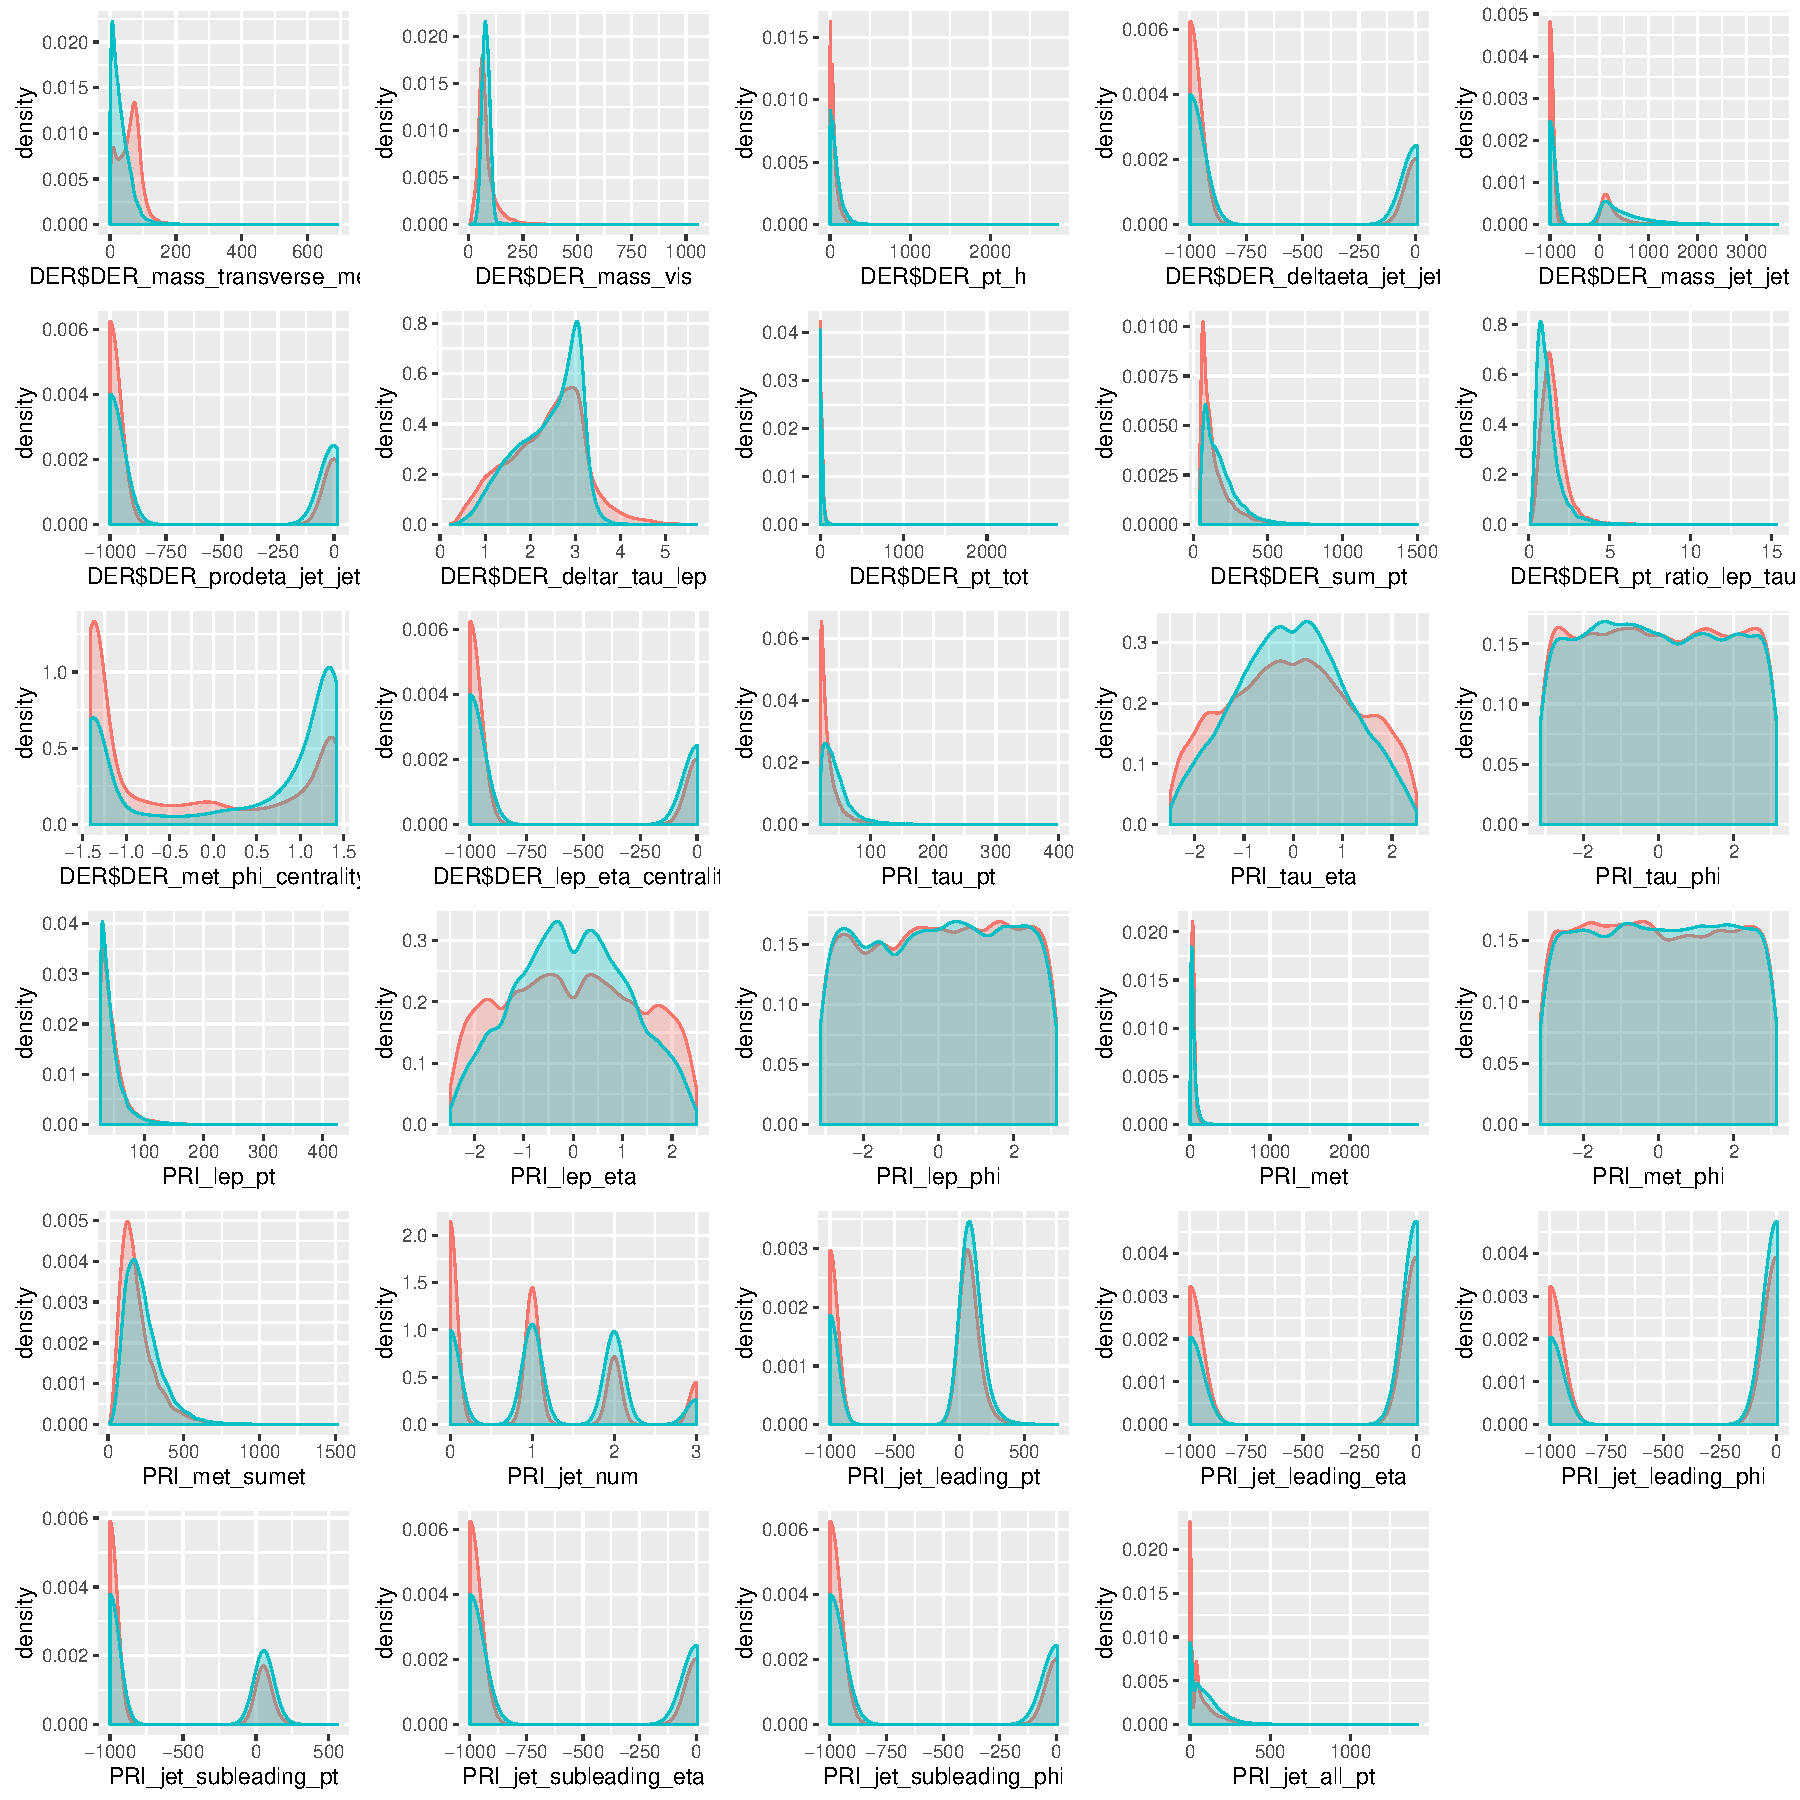
\includegraphics[width=1.05\linewidth]{eda_density_plots.pdf}
\caption{Density plots of features (red = background, blue = signal)}
\end{figure}

\begin{figure}[!ht]
\centering
\begin{minipage}{.5\textwidth}
  \centering
  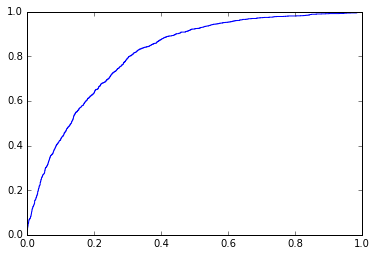
\includegraphics[width=.8\linewidth]{lasso_lr_roc.png}
  \caption{ROC plot of LASSO Logistic Regression}
\end{minipage}%
\begin{minipage}{.5\textwidth}
  \centering
  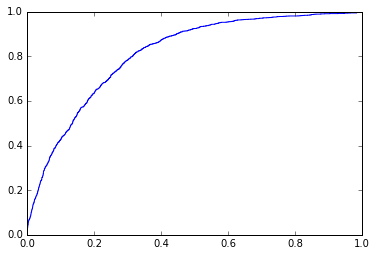
\includegraphics[width=.8\linewidth]{ridge_lr_roc.png}
  \caption{ROC plot of Ridge Logistic Regression}
\end{minipage}%
% \end{figure}

% \begin{figure}[!ht]
\centering
\begin{minipage}{.5\textwidth}
  \centering
  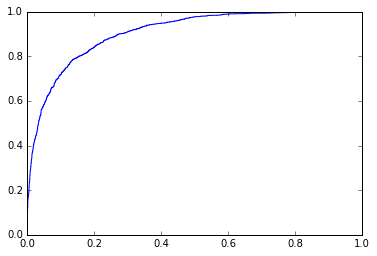
\includegraphics[width=0.8\linewidth]{rf_rocplot.png}
  \caption{ROC plot of Random Forest}
\end{minipage}%
\begin{minipage}{.5\textwidth}
  \centering
  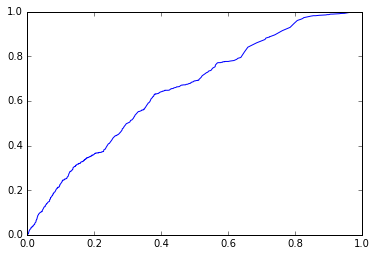
\includegraphics[width=0.8\linewidth]{nb_rocplot.png}
  \caption{ROC plot of Naive Bayes}
\end{minipage}%
% \end{figure}

% \begin{figure}[!ht]
\centering
\begin{minipage}{.5\textwidth}
  \centering
  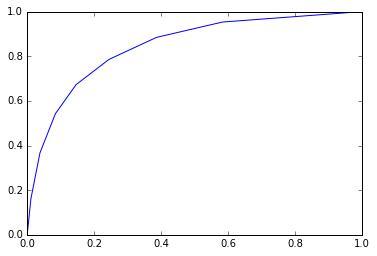
\includegraphics[width=.8\linewidth]{knn_rocplot.png}
  \caption{ROC plot of K-nearst Neighbors}
\end{minipage}%
\begin{minipage}{.5\textwidth}
  \centering
  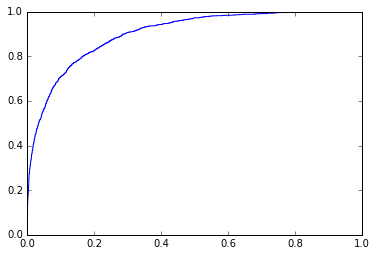
\includegraphics[width=.8\linewidth]{grad_rocplot.png}
  \caption{ROC plot of Gradient Boosting Classifier}
\end{minipage}%
% \end{figure}

% \begin{figure}[!ht]
\centering
\begin{minipage}{.5\textwidth}
  \centering
  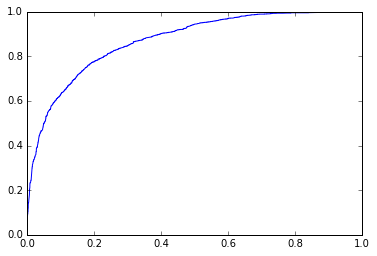
\includegraphics[width=.8\linewidth]{adaboost_rocplot.png}
  \caption{ROC plot of Adaboosting Classifier}
\end{minipage}%
\begin{minipage}{.5\textwidth}
  \centering
  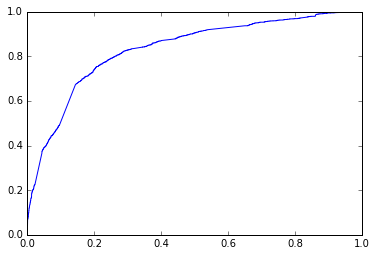
\includegraphics[width=.8\linewidth]{dp_rocplot.png}
  \caption{\small{ROC plot of Deep Learning}}
\end{minipage}%
\end{figure}





%\begin{figure}[ht!]
%\begin{center}
%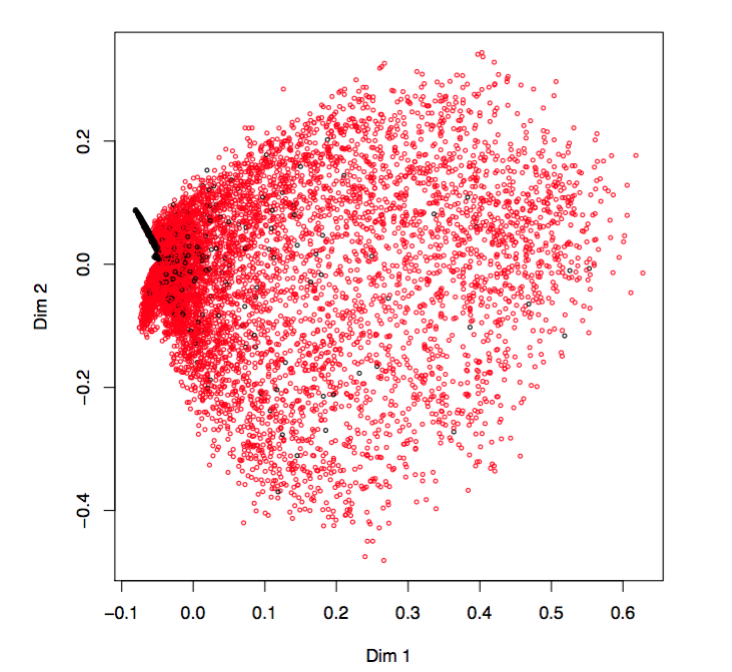
\includegraphics[width=5in]{mds.png}
%\end{center}
%\caption{Random Forest MDS}
%\end{figure}



\end{document}


